%%%%%%%%%%%%%%%%%%%%%%%%%%%%%%%%%%%%%%%%%%%%%%%%%%%%%%%%%%%%%%%%%%% 
%                                                                 %
%                           INLEIDING                             %
%                                                                 %
%%%%%%%%%%%%%%%%%%%%%%%%%%%%%%%%%%%%%%%%%%%%%%%%%%%%%%%%%%%%%%%%%%% 


\chapter{Ontwerpproces}

In dit hoofdstuk worden de ondernomen stappen besproken bij het ontwerpen van een interface die kristalstructuren, in de vorm van een CIF-bestand, kan visualiseren in Blender. Een meer gedetailleerde beschrijving van dit proces kan worden gevonden in hoofdstuk vier, hier wordt ook dieper ingegaan in de installatie van de twee externe programma's, OpenBabel en PyCIFRW, die zullen besproken worden in dit hoofdstuk. De eerste sectie beschrijft hoe de inwendige symmetrie een probleem vormt bij het visualiseren van kristallen, wat het programma OpenBabel doet en hoe het gebruiken hiervan een oplossing biedt op dit probleem.
In de tweede sectie zal worden uitgelegd hoe, met behulp van een parser, een programma in Python kan geschreven worden dat de gegevens uit een CIF-bestand kan omzetten in verwerkbare data en deze opslaat in geschikte datastructuren.


\section{Inwendige symmetrie}

\subsection{Symmetrieoperaties in het CIF-formaat}
Zoals in sectie 2.1.5 van deze tekst staat beschreven kan een kristal worden beschreven aan de hand van een aantal parameters en een lijst van elementen. Dit kan ook gezien worden in het CIF-bestand van Chaziet[Bijlage B] waar slechts vijf atomen worden beschreven terwijl het eenheidskristal in het totaal uit 150 atomen bestaat. Dit is erg handig aangezien er dertig keer zo weinig atomen moeten worden beschreven. In dit onderzoek vormt dit echter een probleem. Om een kristal te tekenen dient natuurlijk de positie van elk element gekend te zijn.
\par
Aan de hand van de ruimtegroep en de centering van het kristalrooster kunnen alle symmetrieoperaties worden verkregen. Deze symmetrieoperaties zijn in het CIF-formaat reeds gegeven in het blok \textit{\_symmetry\_equiv\_pos\_as\_xyz} als een lijst van fractionele coördinaten. Vanuit deze symmetrieoperaties kunnen de posities van elk element in het kristal berekend worden. Er dient rekening gehouden te worden met de mogelijkheid dat één bepaald element aan de hand van verschillende berekeningen kan verkregen worden zodat dit niet meermaals wordt genoteerd, en later getekend. Het is mogelijk een functie te schrijven die de lijst van symmetrieoperaties ophaalt en vervolgens voor elk van deze symmetrieoperaties de positie van de elementen berekenen die ze representeren. Er bestaan echter reeds programma's die dit soort berekeningen kunnen doen, OpenBabel is hier één van.
\par
\subsection{OpenBabel}
OpenBabel is een open source chemische toolbox die gebruikt wordt om chemische data te zoeken, analyseren en te converteren.\citep*{OBAB1} Naast het converteren tussen een groot aantal chemische dataformaten kan OpenBabel ook binnen eenzelfde formaat data converteren. Deze functionaliteit laat onder andere toe de kristaldata van een CIF-bestand om te zetten naar data van datzelfde kristal met een andere ruimtegroep. Door de ruimtegroep aan te passen naar dat van P 1 zal er geen inwendige symmetrie meer bestaan, dit wil zeggen dat elk element dat beschreven wordt slechts op één plaats voorkomt. In plaats van een lange lijst van symmetrieoperaties zal elk element dat gevormd kan worden door deze operaties in het blok met de atoombeschrijvingen komen te staan.   
\par
De broncode van OpenBabel staat vrij beschikbaar op hun GitHub pagina.  Hiernaast is het ook mogelijk de GUI-versie van OpenBabel te downloaden door de installatie-instructies te volgen die te vinden zijn op hun officiële webpagina.\citep*{OBAB1}   
\par
\begin{figure}[h]
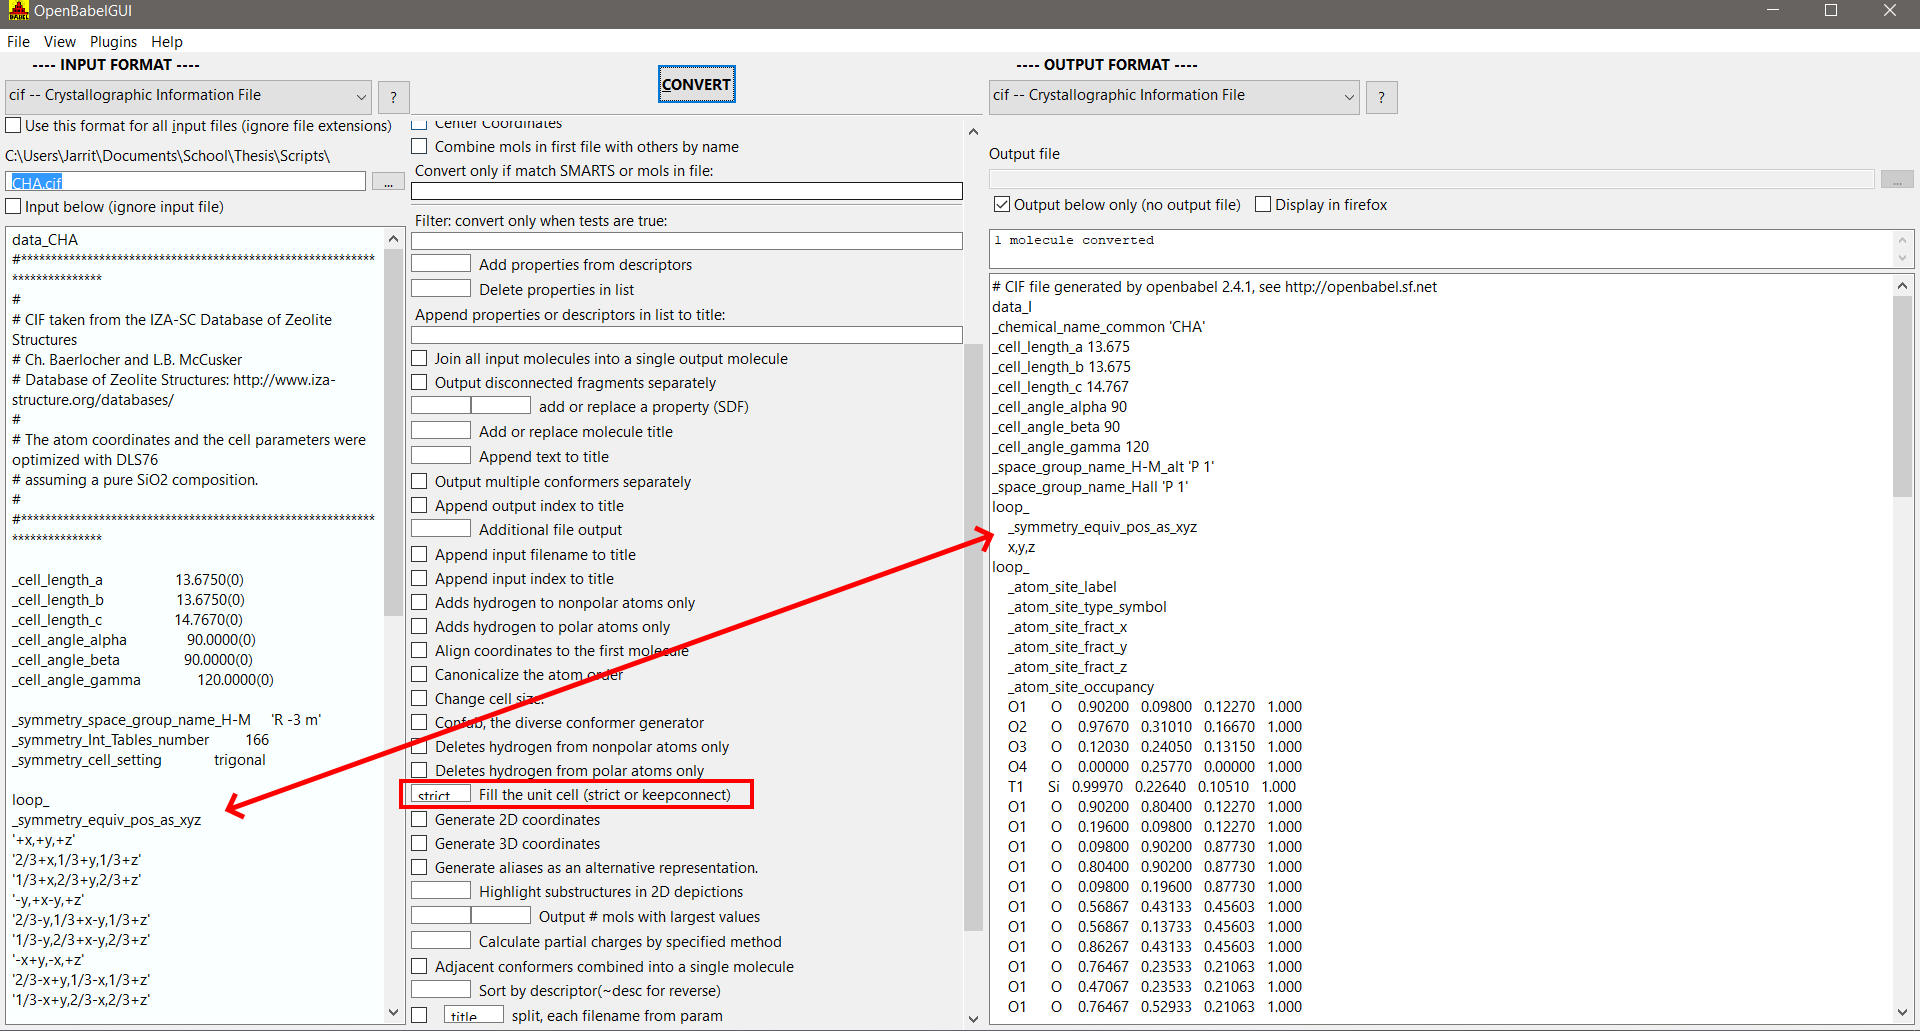
\includegraphics[width=\textwidth,keepaspectratio]{OpenBabelGUI.png}
\caption{Conversie van ruimtegroep met OpenBabel GUI}
\end{figure}
\par
In figuur[3.1] wordt de GUI van OpenBabel afgebeeld. In de linker- en rechterkolom van dit venster staan de in- en uitvoer van het programma en hun formaat. In de middelste kolom kunnen verschillende soorten van conversies worden aangeduid. In het geval van de afbeelding zijn zowel in- als uitvoer in het CIF-formaat en staat het \textit{Fill the unit cel}-vakje op \textit{strict}. Deze opties zorgen ervoor dat het invoerbestand zal worden omgezet naar een ander CIF-bestand maar ditmaal zonder symmetrieoperaties, wat duidelijk wordt bij het bekijken van de twee buitenste kolommen. Bij dit voorbeeld is er maar een optie aangeduid, er zijn nog een groot aantal erg handige keuzemogelijkheden maar deze komen voorlopig niet aan bod.
\par
Hoewel de OpenBabel GUI het converteren van data erg eenvoudig en overzichtelijk maakt, zou het niet erg efficiënt zijn dat dit proces manueel moet worden gedaan voor elk kristal. Deze software kan echter ook vanuit een terminal worden uitgevoerd, wat, in combinatie met de subprocess module van python, de kristallografische interface toelaat deze conversie automatisch te laten verlopen. In hoofdstuk vijf wordt dit in meer detail uitgelegd.
\par     
\section{Van CIF naar py}

\subsection{Ontwerpen van datastructuren}
Nu het CIF-bestand naar een meer bruikbaar formaat is omgezet, is er nood aan datastructuren waarin de informatie kan geparsed worden. Zo een datastructuur noemt men een klasse en het werken hiermee wordt object georiënteerd programmeren genoemd. Enkele voordelen dat dit biedt over de klassieke, imperatieve methode van programmeren, zijn overzichtelijkheid, herbruikbaarheid van klassen en een extra laag van veiligheid doordat de data niet rechtstreeks kan worden aangepast.
\par
Het inlezen van de data wordt in drie klassen gedaan. Een eerste klasse, \textit{Cell}, die informatie bevat over het kristalrooster, waaronder de roosterparameters. Deze data-elementen worden ook wel de attributen van een klasse genoemd. Een tweede klasse, \textit{Atom}, die de fractionele coördinaten van het atoom bevat en welk element het voorstelt. De derde klasse, \textit{Crysdata}, overkoepelt voorgaande klassen in de zin dat deze naast de naam van het kristal ook één object van de klasse \textit{Cell} en een lijst van objecten van de klasse \textit{Atom} bevat. Hiernaast bezit elke klasse ook een methode, \textit{printout}, die de data van de klasse op een nette manier weergeeft op de terminal. Methodes zijn functies die op een object van een klasse kunnen worden opgeroepen.  In Figuur[3.2] worden de onderlinge verhoudingen van deze klassen verduidelijkt, dergelijke figuur wordt een klassendiagramma genoemd, en geeft de algemene opbouw van een programma aan de hand van de gebruikte attributen, methodes, modules en hun onderlinge relaties. Uit dit diagram kan er geïnterpreteerd worden hoe de data uit het CIF-bestand met behulp van de PyCIFRW-parser zal worden ingelezen in de drie eerder genoemde klassen.

\begin{figure}[h]
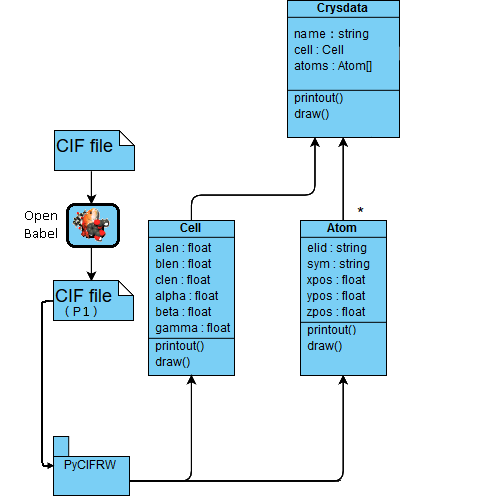
\includegraphics[scale=0.7]{ClassDiagramEz.png}
\caption{Vereenvoudigd klassendiagramma van het programma}
\end{figure}

\subsection{Zelf een parser ontwerpen}
In de vierde sectie van hoofdstuk twee werd er reeds aangehaald wat er allemaal komt kijken bij het ontwerpen van een parser. Het is me gelukt een programma[Bijlage C] te ontwerpen dat alle CIF-bestanden kan inlezen die te vinden zijn op de kristallografische databank van het IZA.\citep*{IZA1} Het parsen van deze bestanden lukte omdat deze allemaal dezelfde tekststructuur hebben. Bestanden uit databanken die werken met een andere structuur kunnen verkeerd worden geïnterpreteerd waardoor de parser nutteloos is. Het is mogelijk mijn parser aan te passen zodat, ongeacht de structuur van het CIF-bestand, een juiste interpretatie van de data kan gedaan worden. Dit zou echter veel tijd vergen en zal, gezien er reeds werkende CIF-parsers bestaan, niet worden gedaan.

PyCIFRW kan eenvoudig worden geïnstaleerd voor python met het commando
pip install PyCifRW 

Door de module \textit{CifFile} te importeren in een pythonscript kan vervolgens nagegaan worden of het programma correct is geïnstalleerd. 

\subsection{Inlezen van CIF-bestanden}
In de vierde sectie van hoofdstuk twee van deze tekst wordt het nut en de werking van een parser besproken. Er wordt ook gekeken naar twee bestaande programma's die in staat zijn CIF-bestanden te parsen en waarom PyCIFRW de voorkeur krijgt in dit onderzoek.
\par
Door de module \textit{CifFile} te importeren kunnen de schrijf- en leesfuncties van PyCIFRW worden opgeroepen in het programma. Nu kan het bestand, dat eerder werd omgezet met behulp van OpenBabel, worden geparsed. De geparsede data zal in de vorm van een soort dictionary ter beschikking zijn. Een dictionary is een python structuur die bestaat uit een lijst van sleutels, \textit{keys}, en hun corresponderende waarden, \textit{values} genoemd. De data kan verkregen worden door de dictionary op te roepen met een bepaalde sleutel.
\par
De sleutels van de dictionary die de PyCIFRW parser aanmaakt stemmen overeen met de namen die te vinden zijn in het CIF-bestand zelf. Op deze manier kan de data dus bekomen worden die vervolgens in de klassen worden ingevuld.

\subsection{Tekenen in Blender}


  






